% Options for packages loaded elsewhere
\PassOptionsToPackage{unicode}{hyperref}
\PassOptionsToPackage{hyphens}{url}
%
\documentclass[
  english,
  man]{apa6}
\usepackage{amsmath,amssymb}
\usepackage{lmodern}
\usepackage{ifxetex,ifluatex}
\ifnum 0\ifxetex 1\fi\ifluatex 1\fi=0 % if pdftex
  \usepackage[T1]{fontenc}
  \usepackage[utf8]{inputenc}
  \usepackage{textcomp} % provide euro and other symbols
\else % if luatex or xetex
  \usepackage{unicode-math}
  \defaultfontfeatures{Scale=MatchLowercase}
  \defaultfontfeatures[\rmfamily]{Ligatures=TeX,Scale=1}
\fi
% Use upquote if available, for straight quotes in verbatim environments
\IfFileExists{upquote.sty}{\usepackage{upquote}}{}
\IfFileExists{microtype.sty}{% use microtype if available
  \usepackage[]{microtype}
  \UseMicrotypeSet[protrusion]{basicmath} % disable protrusion for tt fonts
}{}
\makeatletter
\@ifundefined{KOMAClassName}{% if non-KOMA class
  \IfFileExists{parskip.sty}{%
    \usepackage{parskip}
  }{% else
    \setlength{\parindent}{0pt}
    \setlength{\parskip}{6pt plus 2pt minus 1pt}}
}{% if KOMA class
  \KOMAoptions{parskip=half}}
\makeatother
\usepackage{xcolor}
\IfFileExists{xurl.sty}{\usepackage{xurl}}{} % add URL line breaks if available
\IfFileExists{bookmark.sty}{\usepackage{bookmark}}{\usepackage{hyperref}}
\hypersetup{
  pdftitle={Development of an Intentionally Bi-factor Engagement Measure},
  pdfauthor={Morgan Russell1, Casey Osorio-Duffoo2, Renata Garcia Prieto Palacios Roji1, \& John Kulas1},
  pdflang={en-EN},
  pdfkeywords={Engagement, engagement},
  hidelinks,
  pdfcreator={LaTeX via pandoc}}
\urlstyle{same} % disable monospaced font for URLs
\usepackage{graphicx}
\makeatletter
\def\maxwidth{\ifdim\Gin@nat@width>\linewidth\linewidth\else\Gin@nat@width\fi}
\def\maxheight{\ifdim\Gin@nat@height>\textheight\textheight\else\Gin@nat@height\fi}
\makeatother
% Scale images if necessary, so that they will not overflow the page
% margins by default, and it is still possible to overwrite the defaults
% using explicit options in \includegraphics[width, height, ...]{}
\setkeys{Gin}{width=\maxwidth,height=\maxheight,keepaspectratio}
% Set default figure placement to htbp
\makeatletter
\def\fps@figure{htbp}
\makeatother
\setlength{\emergencystretch}{3em} % prevent overfull lines
\providecommand{\tightlist}{%
  \setlength{\itemsep}{0pt}\setlength{\parskip}{0pt}}
\setcounter{secnumdepth}{-\maxdimen} % remove section numbering
% Make \paragraph and \subparagraph free-standing
\ifx\paragraph\undefined\else
  \let\oldparagraph\paragraph
  \renewcommand{\paragraph}[1]{\oldparagraph{#1}\mbox{}}
\fi
\ifx\subparagraph\undefined\else
  \let\oldsubparagraph\subparagraph
  \renewcommand{\subparagraph}[1]{\oldsubparagraph{#1}\mbox{}}
\fi
% Manuscript styling
\usepackage{upgreek}
\captionsetup{font=singlespacing,justification=justified}

% Table formatting
\usepackage{longtable}
\usepackage{lscape}
% \usepackage[counterclockwise]{rotating}   % Landscape page setup for large tables
\usepackage{multirow}		% Table styling
\usepackage{tabularx}		% Control Column width
\usepackage[flushleft]{threeparttable}	% Allows for three part tables with a specified notes section
\usepackage{threeparttablex}            % Lets threeparttable work with longtable

% Create new environments so endfloat can handle them
% \newenvironment{ltable}
%   {\begin{landscape}\centering\begin{threeparttable}}
%   {\end{threeparttable}\end{landscape}}
\newenvironment{lltable}{\begin{landscape}\centering\begin{ThreePartTable}}{\end{ThreePartTable}\end{landscape}}

% Enables adjusting longtable caption width to table width
% Solution found at http://golatex.de/longtable-mit-caption-so-breit-wie-die-tabelle-t15767.html
\makeatletter
\newcommand\LastLTentrywidth{1em}
\newlength\longtablewidth
\setlength{\longtablewidth}{1in}
\newcommand{\getlongtablewidth}{\begingroup \ifcsname LT@\roman{LT@tables}\endcsname \global\longtablewidth=0pt \renewcommand{\LT@entry}[2]{\global\advance\longtablewidth by ##2\relax\gdef\LastLTentrywidth{##2}}\@nameuse{LT@\roman{LT@tables}} \fi \endgroup}

% \setlength{\parindent}{0.5in}
% \setlength{\parskip}{0pt plus 0pt minus 0pt}

% \usepackage{etoolbox}
\makeatletter
\patchcmd{\HyOrg@maketitle}
  {\section{\normalfont\normalsize\abstractname}}
  {\section*{\normalfont\normalsize\abstractname}}
  {}{\typeout{Failed to patch abstract.}}
\patchcmd{\HyOrg@maketitle}
  {\section{\protect\normalfont{\@title}}}
  {\section*{\protect\normalfont{\@title}}}
  {}{\typeout{Failed to patch title.}}
\makeatother
\shorttitle{BiFactor Engagement}
\keywords{Engagement, engagement\newline\indent Word count: X}
\DeclareDelayedFloatFlavor{ThreePartTable}{table}
\DeclareDelayedFloatFlavor{lltable}{table}
\DeclareDelayedFloatFlavor*{longtable}{table}
\makeatletter
\renewcommand{\efloat@iwrite}[1]{\immediate\expandafter\protected@write\csname efloat@post#1\endcsname{}}
\makeatother
\usepackage{csquotes}
\ifxetex
  % Load polyglossia as late as possible: uses bidi with RTL langages (e.g. Hebrew, Arabic)
  \usepackage{polyglossia}
  \setmainlanguage[]{english}
\else
  \usepackage[main=english]{babel}
% get rid of language-specific shorthands (see #6817):
\let\LanguageShortHands\languageshorthands
\def\languageshorthands#1{}
\fi
\ifluatex
  \usepackage{selnolig}  % disable illegal ligatures
\fi
\newlength{\cslhangindent}
\setlength{\cslhangindent}{1.5em}
\newlength{\csllabelwidth}
\setlength{\csllabelwidth}{3em}
\newenvironment{CSLReferences}[2] % #1 hanging-ident, #2 entry spacing
 {% don't indent paragraphs
  \setlength{\parindent}{0pt}
  % turn on hanging indent if param 1 is 1
  \ifodd #1 \everypar{\setlength{\hangindent}{\cslhangindent}}\ignorespaces\fi
  % set entry spacing
  \ifnum #2 > 0
  \setlength{\parskip}{#2\baselineskip}
  \fi
 }%
 {}
\usepackage{calc}
\newcommand{\CSLBlock}[1]{#1\hfill\break}
\newcommand{\CSLLeftMargin}[1]{\parbox[t]{\csllabelwidth}{#1}}
\newcommand{\CSLRightInline}[1]{\parbox[t]{\linewidth - \csllabelwidth}{#1}\break}
\newcommand{\CSLIndent}[1]{\hspace{\cslhangindent}#1}

\title{Development of an Intentionally Bi-factor Engagement Measure}
\author{Morgan Russell\textsuperscript{1}, Casey Osorio-Duffoo\textsuperscript{2}, Renata Garcia Prieto Palacios Roji\textsuperscript{1}, \& John Kulas\textsuperscript{1}}
\date{}


\authornote{

Add complete departmental affiliations for each author here. Each new line herein must be indented, like this line.

Enter author note here.

Correspondence concerning this article should be addressed to Morgan Russell, 1 Normal Ave, Montclair, NJ 07043. E-mail: \href{mailto:russellm5@montclair.edu}{\nolinkurl{russellm5@montclair.edu}}

}

\affiliation{\vspace{0.5cm}\textsuperscript{1} Montclair State University\\\textsuperscript{2} Harver}

\abstract{
Employee engagement has enjoyed a surge in interest as a positive employee outcome despite continued disageement regarding its factor structure and nomological relationship to other constructs, like burnout.
We contrast two three-factor models of engagement: substantive, with the dimensions vigor, dedication and absorption, and attitudinal, with cognitive, affective and behavioral dimensions.
Using bifactor analysis, study 1 proposes a scale that reconciles these two models and reduces 36 candidate items to 18.
Study 2 convergently and discriminantly validates this scale.
}



\begin{document}
\maketitle

\#Introduction

\begin{quote}
Renata's SEM paper will come in handy
\end{quote}

Recent decades have seen a proliferation of interest and research in the construct of employee engagement.

\begin{quote}
more on why we're looking at tripartite model
\end{quote}

The roots of employee (aka work; e.g., W. Schaufeli \& Bakker, 2010) engagement research likely started with theoretical expansions of forms of employee participation (see, for example, Ferris \& Hellier, 1984) and job involvement (e.g., Elloy, Everett, \& Flynn, 1991). This exploration extended into broader considerations of attitudes and emotions (Staw, Sutton, \& Pelled, 1994) and were informed by further exploration of the dimensionality of constructs such as organizational commitment (Meyer \& Allen, 1991). The 1990's saw focused development and refinement (for example, a dissertation; Leone (1995) or actual semantic reference; William A. Kahn (1990a)). Staw, Sutton, and Pelled (1994) investigated the relationships between \emph{positive emotions} and favorable work outcomes, and although they do not use the word, ``engagement,'' their distinction between felt and expressed emotion likely held influence upon the burgeoning interest in the engagement construct.

\begin{quote}
burnout
\end{quote}

Although occasionally referred to as residing on the opposing pole to \emph{burnout} (Christina Maslach \& Leiter, 2008), these two constructs are currently most commonly conceptualized as being distinct (Goering, Shimazu, Zhou, Wada, \& Sakai, 2017; Kim, Shin, \& Swanger, 2009; Wilmar B. Schaufeli, Taris, \& Van Rhenen, 2008; Timms, Brough, \& Graham, 2012), although certainly not universally (Cole, Walter, Bedeian, \& O'Boyle, 2012; Taris, Ybema, \& Beek, 2017). Comparing the two, Goering, Shimazu, Zhou, Wada, and Sakai (2017) concluded that they have a moderate (negative) association, but also distinct nomological networks. Wilmar B. Schaufeli, Taris, and Van Rhenen (2008) investigated both internal and external association indicators, concluding that engagement and burnout (as well as \emph{workaholism}) should be considered three distinct constructs.

Burnout can be defined as a psychological syndrome characterized by exhaustion (low energy), cynicism (low involvement), and inefficacy (low self-efficacy), which is experienced in response to chronic job stressors (e.g., Leiter \& Maslach, 2004; C. Maslach \& Leiter, 1997). Alternatively, engagement refers to an individual worker's involvement and satisfaction as well as enthusiasm for work (Harter, Schmidt, \& Hayes, 2002). W. B. Schaufeli and Bakker (2003) further specify a ``positive, fulfilling, work-related state of mind that is characterized by vigor, dedication, and absorption'' (p.~74). Via their conceptualization, vigor is described as high levels of energy and mental resilience while working. Dedication refers to being strongly involved in one's work and experiencing a sense of significance, enthusiasm, inspiration, pride, and challenge. Absorption is characterized by being fully concentrated and happily engrossed in one's work, whereby time passes quickly and one has difficulties with detaching oneself from work (Wilmar B. Schaufeli, Salanova, González-Romá, \& Bakker, 2002). The dimension of absorption has been noted as being influenced in conceptual specification by (Csikszentmihalyi, 1990)'s concept of ``flow.''

Regarding measurement, Gallup is widely acknowledged as an early pioneer in the measurement of the construct (see, for example, Coffman \& Harter, 1999). The Utrecht Work Engagement Scale (UWES) is another self-report questionnaire developed by W. B. Schaufeli and Bakker (2003) that directly assesses the vigor, dedication, and absorption elements.

\begin{quote}
TRIPARTITE MODEL--work here
\end{quote}

The first, to our knowledge, use of the word ``engagement'' as a construct came from William A. Kahn (1990b), who defined it as: ``the harnessing of organization members' selves to their work roles; in engagement, people employ and express themselves physically, cognitively, and emotionally during role performances.'' Although this definition was quickly bypassed by subsequent papers (see, for example, (Baumruk, 2004) and (Shaw, 2005), who framed it in terms of one's cognitive and affective \emph{commitment} to one's organization), William A. Kahn (1990b)'s definition is notable in that it conforms to the then-ascendant tripartite model of attitudes proposed by Rosenberg (1960). This model frames attitudes as latent variables that manifest cognitively, affectively and behaviorally.

Although falling out of favor in the decades following its construction, interest in the tripartite model was revived by Kaiser and Wilson (2019),

\begin{quote}
we need to do some market research on the Q12: 1. what's the feedback report look like? (google images show one overall ``satsifaction'' score and/or one overall ``engagement'' score), 2. how much does it cost, 3. what are the 200 pulse items Gallup refers to? (6/7/21)
\end{quote}

Our conceptualization of work engagement is a mental state wherein employees\ldots{}

\begin{itemize}
\tightlist
\item
  \ldots feel energized (\textbf{Vigor})
\item
  \ldots are enthusiastic about the content of their work and the things they do (\textbf{Dedication})
\item
  \ldots are so immersed in their work activities that time seems compressed (\textbf{Absorption})
\end{itemize}

This model is not without criticism, however. Some critics question its structural validity by pointing out that vigor, dedication and absorption all correlate highly with each other (Kulikowski, 2017).

\begin{quote}
need more on criticisms of model
\end{quote}

The present article explores two methods for constructing a scale that incorporates both the substantive and attitudinal models into one, a more classical one based on corrected item-total correlations and one based on modification indices.

\hypertarget{methods}{%
\section{Methods}\label{methods}}

Choice of focus on BIC versus AIC discussed in Dziak, Coffman, Lanza, Li, and Jermiin (2020).

\begin{verbatim}
##   [1] 2 3 1 2 3 2 1 1 2 2 2 3 1 1 3 2 3 2 3 1 1 3 1 3 2 2 1 2 2 1 2 3 2 2 2 4 2
##  [38] 3 3 3 2 2 3 2 1 3 1 2 3 2 1 2 2 1 2 3 3 1 1 2 2 1 2 2 3 2 1 2 3 2 3 2 1 7
##  [75] 1 2 2 2 1 2 2 1 3 2 4 2 8 2 2 3 5 2 1 2 3 2 2 2 1 2 1 3 3 2 3 2 2 2 3 3 2
## [112] 2 2 1 2 2 3 2 5 2 3 2 3 2 3 3 1 2 1 3 8 2 1 3 2 3 3 5 3 2 2 2 2 1 3 2 3 3
## [149] 5 2 2 3 2 1 2 3 1 2 3 4 1 2 1 2 1 2 3 5 2 3 2 2 1 3 5 8 5 2 2 3 3 2 1 2 2
## [186] 3 1 1 3 3 1 2 2 2 1 2 2 2 2 3 2 3 2 2 2 2 1 3 3 4 2 2 2 3 1 2 2 1 2 1 2 1
## [223] 1 2 5 2 2 1 2 2 2 2 1 2 3 3 1 3 2 2 2 2 1 2 2 2 3 3 2
\end{verbatim}

\hypertarget{participants}{%
\subsection{Participants}\label{participants}}

330 individuals provided ratings across 36 candidate items. These participants were gathered via snowball sampling, with an initial population of undergraduate and graduate students, as well as professional acquaintances of faculty members.` All surveys were administered on Qualtrics.

Participant job title, hours worked per week, and organizational tenure were recorded. Mean hours worked per week was 40.59 (SD = 13.69), see Figure \ref{fig:hours}. Mean organizational tenure was 6.82 (SD = 8.50), see Figure \ref{fig:tenure}. Participants who did not exactly specify their tenure (e.g.~``A bit over a year'') were not included in this average.

\begin{figure}
\centering
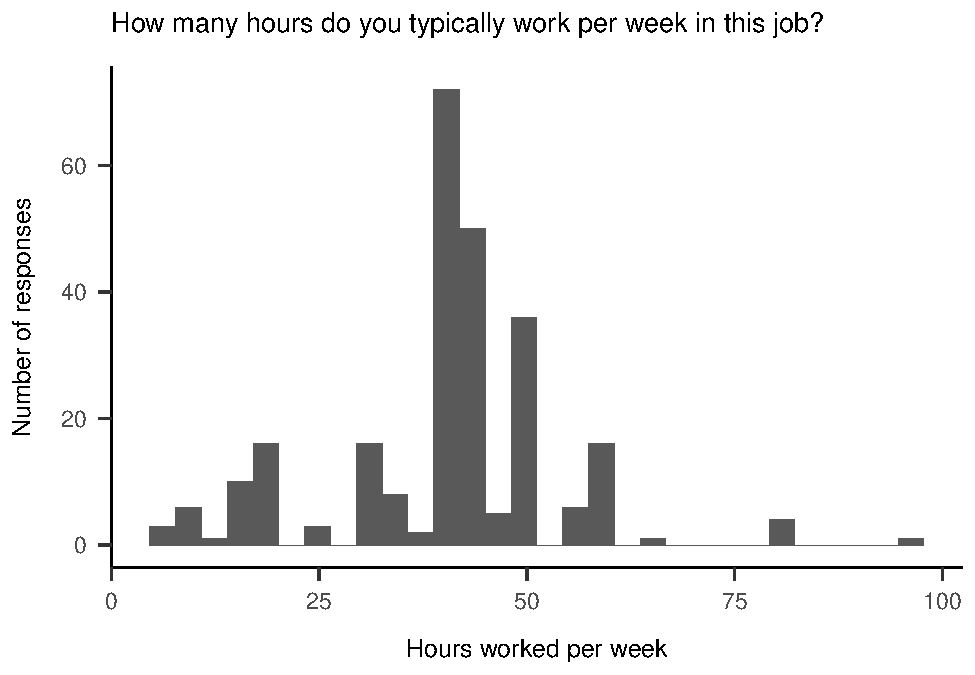
\includegraphics{SIOPpapaja_files/figure-latex/hours-1.pdf}
\caption{\label{fig:hours}Distribution of mean hours worked per week}
\end{figure}

\begin{figure}
\centering
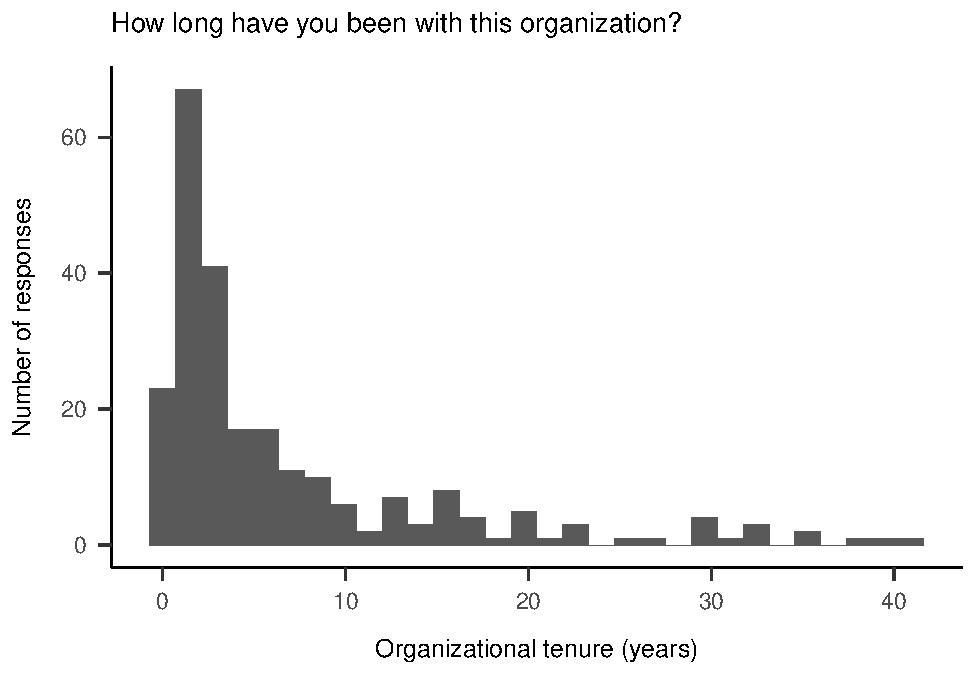
\includegraphics{SIOPpapaja_files/figure-latex/tenure-1.pdf}
\caption{\label{fig:tenure}Distribution of organizational tenure (years)}
\end{figure}

Participants provided their job titles via an optional free text-entry box at the end of the survey. From there, we classified job titles according to the International Standard Classification of Occupations (ISCO-8) with the \texttt{classify\_occupation} function within the \texttt{labourR} package ((\textbf{kouretsis2020?})). The ISCO hierarchically organizes jobs in increasing order of specificity. For example, the first level of the hierarchy distinguishes a professional from a clerical worker or a technician. On the second level, professionals are distinguished among each other by whether they are engineers, medical workers, lawyers, and so on. See \ref{fig:jobs}

\begin{tabular}{l|r}
\hline
Professional category & Count\\
\hline
Clerical Support Workers & 4\\
\hline
Craft and related trades workers & 1\\
\hline
Managers & 51\\
\hline
Plant and machine operators, and assemblers & 3\\
\hline
Professionals & 120\\
\hline
Service and sales workers & 8\\
\hline
Technicians and associate professionals & 62\\
\hline
\end{tabular}

\hypertarget{item-generation}{%
\subsubsection{Item generation}\label{item-generation}}

We generated a set of 50 items for our engagement measure, with the ultimate goal of reducing them to a final set of 18. These items were generated according to a review of extant tripartite engagement measures, as well as \emph{WHAT RESEARCH DID WE USE FOR ATTITUDINAL WORDING? WAS IT LITERALLY JUST ``I THINK,'' ``I FEEL,'' ``I DO?''} Each item was worded to reflect both a substantive dimension as well as an attitudinal dimension. For example, the item ``My job makes me feel like I'm part of something meaningful'' reflects the affective dimension with ``feel'' and the dedication dimension with ``I'm part of something meaningful.''

Our 3x3 bifactor model produced nine pairs of dimensions (e.g., Vigor-Cognitive, Vigor-Affective, Vigor-Behavioral, etc.). With 36 initial items, this left four items per pair of substantive and attitudinal dimensions.

\hypertarget{content-validation-and-initial-item-reduction}{%
\subsubsection{Content validation and initial item reduction}\label{content-validation-and-initial-item-reduction}}

An item sorting process was conducted to ensure content validity of our scale. Our original 50 items were presented to seven masters and PhD students in industrial-organizational psychology at Montclair State University, with each student instructed to sort each item into its respective substantive and attitudinal dimensions. Items that were not sorted into the same substantive-attitudinal dimension pair by at least five of seven raters were excluded from further analysis. Students were not aware of the intended dimensions of each item and were presented with the following definitions for sorting:

Substantive:

\begin{itemize}
\item
  \emph{Absorption}: Being fully immersed in one's work, where time passes quickly and one has difficulty detaching from work tasks
\item
  \emph{Vigor}: Experiencing persistent levels of energy, effort, and enthusiasm while working
\item
  \emph{Dedication}: Experiencing pride and challenge in ones work, as well as strong feelings of support from and loyalty toward the organization
\end{itemize}

Attitudinal:

\begin{itemize}
\item
  \emph{Cognitive}: Pertaining to thoughts or general mental processes (for example what someone thinks)
\item
  \emph{Affective}: Pertaining to feelings or emotions (for example, how someone feels)
\item
  \emph{Behavioral}: Pertaining to acts or actions (for example, what someone does)
\end{itemize}

\begin{quote}
See table \emph{X} for a full list of items and their respective dimensions.
\end{quote}

Following item sorting, we further reviewed the wording of each item and eliminated all that, upon review, fell outside of the content domain (e.g.~``I would rather work here than elsewhere''), eventually arriving at 36 candidate items.

\hypertarget{procedure}{%
\subsection{Procedure}\label{procedure}}

\begin{quote}
Looking into the specification of polychoric covariances (Jöreskog, 1994). This seems to be not very commonly leveraged (only package that seems to estimate these is \texttt{semPlot}).
\end{quote}

The effective result of this was two divergent quasi-experimental approaches: 1) focus on corrected item-total correlations, and 2) focus on CFA modification indices.

\hypertarget{corrected-item-total-correlations}{%
\subsubsection{Corrected item-total correlations}\label{corrected-item-total-correlations}}

\begin{quote}
To Casey: document your process here
\end{quote}

We conducted a correct item-total correlation on our original 36-items set. Base off, the r. drops that the corrected item-total correlations provide us we narrowed it down by selecting that items that had the best r. drops off removing one item at a time. For example, each cell division contain 4 items, therefore, we remove one of the four items creating 6 potential 3 item corrected item correlations, and from there we choose the items with the best r. drops. We continued the same process when narrowing our three items down to two items. An example is shown below:

\hypertarget{cfa-modification-indices}{%
\subsubsection{CFA Modification Indices}\label{cfa-modification-indices}}

We followed two parallel stepwise item-reduction processes centered around eliminating items in decreasing order of modification indices. Looking at the 36-item substantive and attitudinal models independently (process 1 and process 2), we requested modification indices from each, with the intent of retaining indicators whose fixed shared residual covariances were associated with high modification indices (indicating better model fit if the paths were freed). The item pair with the highest modification index was scrutinized, with a subjective group judgment made on wording and content domain coverage. The less preferred item was removed from the model. In cases where the highest modification index was between the only two remaining items in a substantive-attitudinal pair, these items were passed over for scrutiny in favor of the items with the next-highest index. This process was repeated until 18 items remained (i.e., 2 items for each of the 9 substantive-attitudinal pairs).

For example, the path with the highest modification index across both CFAs was between item 2 and item 4, which are both indicators of ``Absorption'' and ``Cognition.'' One of these items was therefore a candidate for deletion, and semantic preference was given to item 4, ``I find it difficult to mentally disconnect from work'' over item 2. After item 2 was excluded from both scale definitions (substantive and attitudinal), the CFAs were re-run and modification indices re-checked for bi-factor structure optimizing modifications.\footnote{Probably put a table in here highlighting certain modification indices (with a key to intended factor-item association). Look at ``modincides1''}

The end result was two separate final scale definitions (one optimized for the substantive model and one for the attitudinal model).

\begin{quote}
Old text: We prioritized item deletions such that an item was implicated for deletion if: 1) modification index was high (relative to others) and 2) error residual was within the same ``cell.'' The choice of item to delete was based on author preference for wording/semantics as well as construct element coverage (considering the possible consequences for construct deficiency). Item variance was also consulted (retention more likely with greater item variance).
\end{quote}

\begin{table}[tbp]

\begin{center}
\begin{threeparttable}

\caption{\label{tab:modindices}Attitudinal structure modification indices (36 item analysis)}

\begin{tabular}{m{2cm}m{2cm}m{2cm}m{7cm}}
\toprule
Element 1 & \multicolumn{1}{c}{Element 2} & \multicolumn{1}{c}{Modification Index} & \multicolumn{1}{c}{Notes}\\
\midrule
Item\_2 & Item\_4 & 192.41 & Candidate for deletion due to construct duplication\\
Item\_8 & Item\_18 & 96.05 & \\
Item\_29 & Item\_35 & 62.25 & Candidate for retention due to substantive construct association\\
Item\_14 & Item\_20 & 56.38 & \\
Item\_1 & Item\_12 & 51.39 & \\
Item\_1 & Item\_13 & 50.33 & \\
Item\_13 & Item\_12 & 41.40 & \\
\bottomrule
\end{tabular}

\end{threeparttable}
\end{center}

\end{table}

\begin{quote}
\begin{quote}
Actually it doesn't matter that much with only 1 item deletion - probably go ahead and do a few before recheck modification indices
\end{quote}
\end{quote}

\hypertarget{single-factor-versus-bifactor-approaches}{%
\subsubsection{Single factor versus bifactor approaches}\label{single-factor-versus-bifactor-approaches}}

\begin{quote}
Casey this is where you come in
\end{quote}

\hypertarget{data-analysis}{%
\subsection{Data analysis}\label{data-analysis}}

We used R {[}Version 4.1.1; R Core Team (2021){]} and the R-packages \emph{apaTables} {[}Version 2.0.8; Stanley (2021){]}, \emph{dplyr} {[}Version 1.0.7; Wickham, François, Henry, and Müller (2021){]}, \emph{DT} {[}Version 0.19; Xie, Cheng, and Tan (2021){]}, \emph{forcats} {[}Version 0.5.1; Wickham (2021a){]}, \emph{ggplot2} {[}Version 3.3.5; Wickham (2016){]}, \emph{kableExtra} {[}Version 1.3.4; Zhu (2021){]}, \emph{labourR} {[}Version 1.0.0; Kouretsis, Bampouris, Morfiris, and Papageorgiou (2020){]}, \emph{lavaan} {[}Version 0.6.9; Rosseel (2012){]}, \emph{magrittr} {[}Version 2.0.1; Bache and Wickham (2020){]}, \emph{papaja} {[}Version 0.1.0.9997; Aust and Barth (2020){]}, \emph{purrr} {[}Version 0.3.4; Henry and Wickham (2020){]}, \emph{readr} {[}Version 2.0.1; Wickham and Hester (2020){]}, \emph{sem} {[}Version 3.1.11; Fox, Nie, and Byrnes (2020); Epskamp (2019){]}, \emph{semPlot} {[}Version 1.1.2; Epskamp (2019){]}, \emph{stringr} {[}Version 1.4.0; Wickham (2019){]}, \emph{tibble} {[}Version 3.1.4; Müller and Wickham (2021){]}, \emph{tidyr} {[}Version 1.1.3; Wickham (2021b){]}, and \emph{tidyverse} {[}Version 1.3.1; Wickham et al. (2019){]} for all our analyses.

\hypertarget{results}{%
\section{Results}\label{results}}

CFA drafts below

\begin{figure}
\centering
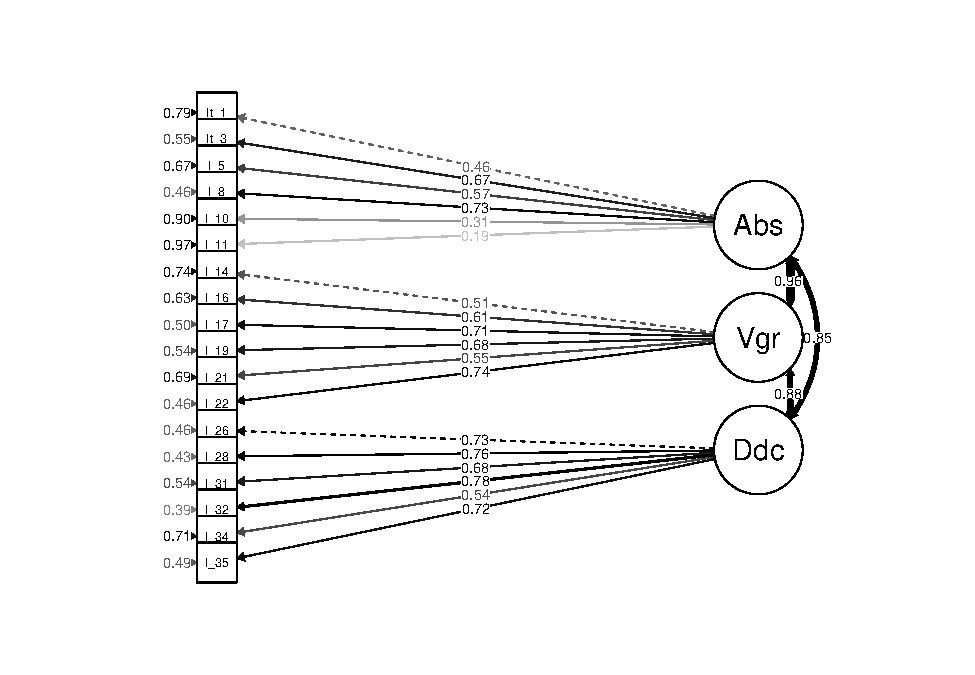
\includegraphics{SIOPpapaja_files/figure-latex/CFAatt1-1.pdf}
\caption{\label{fig:CFAatt1}Substantive factor measurement model}
\end{figure}

\begin{figure}
\centering
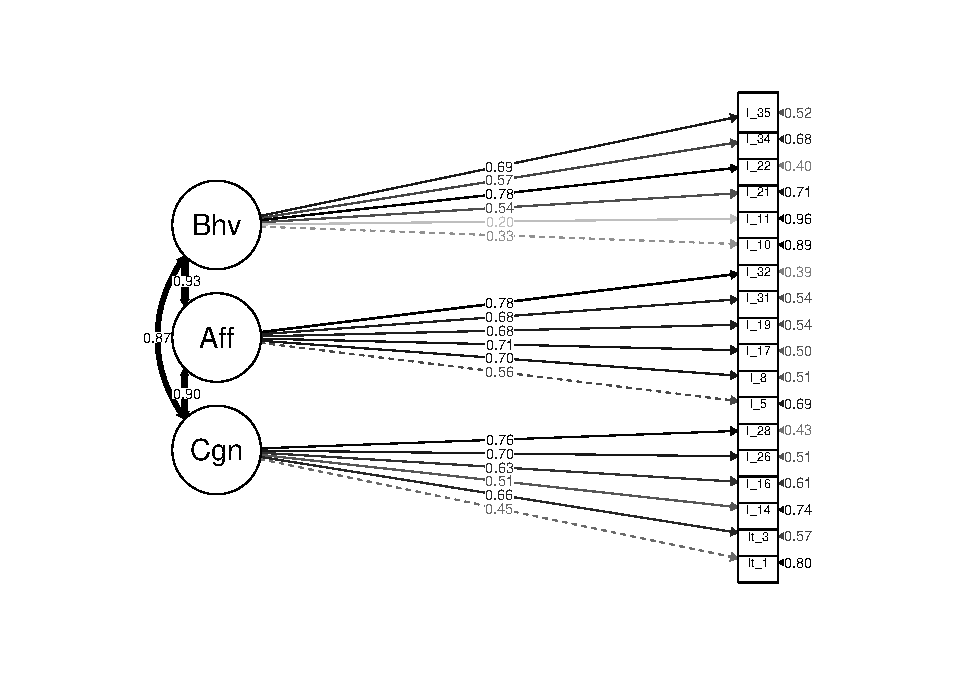
\includegraphics{SIOPpapaja_files/figure-latex/CFAatt2-1.pdf}
\caption{\label{fig:CFAatt2}Attitudinal factor measurement model}
\end{figure}

\begin{figure}
\centering
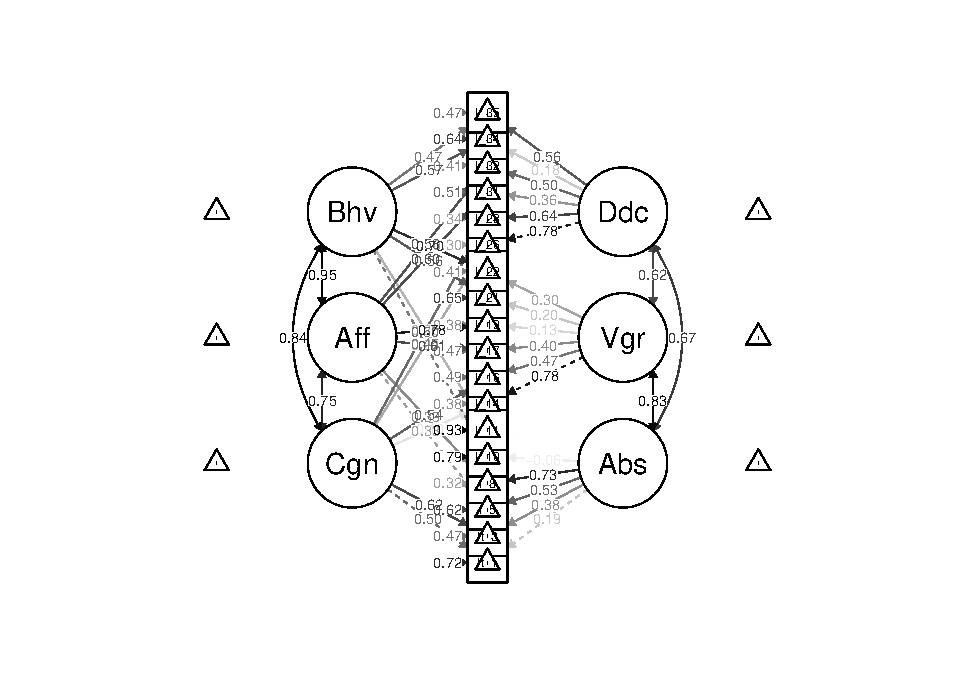
\includegraphics{SIOPpapaja_files/figure-latex/CFAatt3-1.pdf}
\caption{\label{fig:CFAatt3}Bifactor measurement model}
\end{figure}

\begin{table}[tbp]

\begin{center}
\begin{threeparttable}

\caption{\label{tab:fitmeasures}Summary fit statistics (18 item proposed scale definitions)}

\begin{tabular}{llllllll}
\toprule
model & \multicolumn{1}{c}{Chi Square} & \multicolumn{1}{c}{df} & \multicolumn{1}{c}{RMSEA} & \multicolumn{1}{c}{SRMR} & \multicolumn{1}{c}{CFI} & \multicolumn{1}{c}{TLI} & \multicolumn{1}{c}{AIC}\\
\midrule
Attitudinal & 454.30 & 132.00 & 0.10 & 0.07 & 0.83 & 0.80 & 13,473.40\\
Substantive & 473.56 & 132.00 & 0.10 & 0.07 & 0.82 & 0.79 & 13,492.66\\
bifactor & 264.70 & 111.00 & 0.07 & 0.05 & 0.92 & 0.89 & 14,113.31\\
\bottomrule
\end{tabular}

\end{threeparttable}
\end{center}

\end{table}

\hypertarget{study-2}{%
\subsection{Study 2}\label{study-2}}

Construct validation was acccomplished via administration of the 17-item UWES as well as the Saks (2006) 12-item scale. Saks (2006) aggregates to two scales: job and organizational engagement.

\hypertarget{discussion}{%
\section{Discussion}\label{discussion}}

The purpose of this study was to present two divergent approaches for constructing scales that simultaneously probe the substantive and attitudinal factor structures of employee engagement. Toward this end, we propose two similar scale definitions

Our next endeavor will be to establish convergent and discriminant validity of the scales.

Currently, the UWES is one of the most popular engagement scales
Our proposed scale would

Bifactor analysis may be a valuable method of reconciling previously at-odds approaches to describing the same construct.

Our research contributes to theory in two key ways. Firstly, it introduces a novel measure of engagement, developed in English, that will allow future researchers to further probe the tripartite attitudinal structure of the construct. To our knowledge, ours is the only engagement scale that probes the specific attitudinal dimensions of engagement.
Secondly, we more generally advance the use of bifactor analysis as an alternative approach to testing and comparing structural models of constructs. Rather than
We show that a scale can exhibit high internal consistency while simultaneously measuring two different structural models.
It is our hope that the success of this approach might evangelize bifactor analysis and the more general approach of consolidating and integrating theories rather than parsing them.

\newpage

\hypertarget{references}{%
\section{References}\label{references}}

\begingroup
\setlength{\parindent}{-0.5in}
\setlength{\leftskip}{0.5in}

\hypertarget{refs}{}
\begin{CSLReferences}{1}{0}
\leavevmode\hypertarget{ref-R-papaja}{}%
Aust, F., \& Barth, M. (2020). \emph{{papaja}: {Create} {APA} manuscripts with {R Markdown}}. Retrieved from \url{https://github.com/crsh/papaja}

\leavevmode\hypertarget{ref-R-magrittr}{}%
Bache, S. M., \& Wickham, H. (2020). \emph{Magrittr: A forward-pipe operator for r}. Retrieved from \url{https://CRAN.R-project.org/package=magrittr}

\leavevmode\hypertarget{ref-baumruk2004missing}{}%
Baumruk, R. (2004). The missing link: The role of employee engagement in business success, \emph{47}, 48--52.

\leavevmode\hypertarget{ref-coffman_hard_1999}{}%
Coffman, C., \& Harter, J. (1999). A hard look at soft numbers. \emph{Position Paper, Gallup Organization}.

\leavevmode\hypertarget{ref-cole2012job}{}%
Cole, M. S., Walter, F., Bedeian, A. G., \& O'Boyle, E. H. (2012). Job burnout and employee engagement: A meta-analytic examination of construct proliferation. \emph{Journal of Management}, \emph{38}(5), 1550--1581.

\leavevmode\hypertarget{ref-csikszentmihalyi1990flow}{}%
Csikszentmihalyi, M. (1990). \emph{Flow: The psychology of optimal experience} (Vol. 1990). Harper \& Row New York.

\leavevmode\hypertarget{ref-dziak2020sensitivity}{}%
Dziak, J. J., Coffman, D. L., Lanza, S. T., Li, R., \& Jermiin, L. S. (2020). Sensitivity and specificity of information criteria. \emph{Briefings in Bioinformatics}, \emph{21}(2), 553--565.

\leavevmode\hypertarget{ref-elloy_examination_1991}{}%
Elloy, D. F., Everett, J. E., \& Flynn, W. R. (1991). An examination of the correlates of job involvement. \emph{Group \& Organization Studies}, \emph{16}(2), 160--177. \url{https://doi.org/10.1177/105960119101600204}

\leavevmode\hypertarget{ref-R-semPlot}{}%
Epskamp, S. (2019). \emph{semPlot: Path diagrams and visual analysis of various SEM packages' output}. Retrieved from \url{https://CRAN.R-project.org/package=semPlot}

\leavevmode\hypertarget{ref-ferris_added_1984}{}%
Ferris, R., \& Hellier, P. (1984). Added value productivity schemes and employee participation. \emph{Asia Pacific Journal of Human Resources}, \emph{22}(4), 35--44. \url{https://doi.org/10.1177/103841118402200406}

\leavevmode\hypertarget{ref-R-sem}{}%
Fox, J., Nie, Z., \& Byrnes, J. (2020). \emph{Sem: Structural equation models}. Retrieved from \url{https://CRAN.R-project.org/package=sem}

\leavevmode\hypertarget{ref-goering2017not}{}%
Goering, D. D., Shimazu, A., Zhou, F., Wada, T., \& Sakai, R. (2017). Not if, but how they differ: A meta-analytic test of the nomological networks of burnout and engagement. \emph{Burnout Research}, \emph{5}, 21--34.

\leavevmode\hypertarget{ref-harter_business-unit-level_2002}{}%
Harter, J. K., Schmidt, F. L., \& Hayes, T. L. (2002). Business-unit-level relationship between employee satisfaction, employee engagement, and business outcomes: A meta-analysis. \emph{Journal of Applied Psychology}, \emph{87}(2), 268.

\leavevmode\hypertarget{ref-R-purrr}{}%
Henry, L., \& Wickham, H. (2020). \emph{Purrr: Functional programming tools}. Retrieved from \url{https://CRAN.R-project.org/package=purrr}

\leavevmode\hypertarget{ref-joreskog1994estimation}{}%
Jöreskog, K. G. (1994). On the estimation of polychoric correlations and their asymptotic covariance matrix. \emph{Psychometrika}, \emph{59}(3), 381--389.

\leavevmode\hypertarget{ref-kahn1990psychological}{}%
Kahn, William A. (1990b). Psychological conditions of personal engagement and disengagement at work. \emph{Academy of Management Journal}, \emph{33}(4), 692--724.

\leavevmode\hypertarget{ref-kahn_psychological_1990}{}%
Kahn, William A. (1990a). Psychological conditions of personal engagement and disengagement at work. \emph{Academy of Management Journal}, \emph{33}(4), 692--724.

\leavevmode\hypertarget{ref-kaiser_campbell_2019}{}%
Kaiser, F. G., \& Wilson, M. (2019). The {Campbell} {Paradigm} as a {Behavior}-{Predictive} {Reinterpretation} of the {Classical} {Tripartite} {Model} of {Attitudes}. \emph{European Psychologist}, \emph{24}(4), 359--374. \url{https://doi.org/10.1027/1016-9040/a000364}

\leavevmode\hypertarget{ref-kim_burnout_2009}{}%
Kim, H. J., Shin, K. H., \& Swanger, N. (2009). Burnout and engagement: {A} comparative analysis using the {Big} {Five} personality dimensions. \emph{International Journal of Hospitality Management}, \emph{28}(1), 96--104. \url{https://doi.org/10.1016/j.ijhm.2008.06.001}

\leavevmode\hypertarget{ref-R-labourR}{}%
Kouretsis, A., Bampouris, A., Morfiris, P., \& Papageorgiou, K. (2020). \emph{labourR: Classify multilingual labour market free-text to standardized hierarchical occupations}. Retrieved from \url{https://CRAN.R-project.org/package=labourR}

\leavevmode\hypertarget{ref-kulikowski2017we}{}%
Kulikowski, K. (2017). Do we all agree on how to measure work engagement? Factorial validity of utrecht work engagement scale as a standard measurement tool--a literature review. \emph{International Journal of Occupational Medicine and Environmental Health}, \emph{30}(2), 161--175.

\leavevmode\hypertarget{ref-leiter_areas_2004}{}%
Leiter, M., \& Maslach, C. (2004). Areas of worklife: A structured approach to organizational predictors of job burnout. In \emph{Research in occupational stress and well-being} (Vol. 3, pp. 91--134). \url{https://doi.org/10.1016/S1479-3555(03)03003-8}

\leavevmode\hypertarget{ref-leone_relation_1995}{}%
Leone, D. R. (1995). \emph{The relation of work climate, higher order need satisfaction, need salience, and causality orientations to work engagement, psychological adjustment, and job satisfaction} (PhD thesis). ProQuest Information \& Learning.

\leavevmode\hypertarget{ref-maslach1997causes}{}%
Maslach, C., \& Leiter, M. (1997). What causes burnout. \emph{Maslach C, Leiter MP. The Truth About Burnout: How Organizations Cause Personal Stress and What to Do about It. San Francisco, CA: Josey-Bass Publishers}, 38--60.

\leavevmode\hypertarget{ref-maslach_early_2008}{}%
Maslach, Christina, \& Leiter, M. P. (2008). Early predictors of job burnout and engagement. \emph{Journal of Applied Psychology}, \emph{93}(3), 498--512.

\leavevmode\hypertarget{ref-meyer_three-component_1991}{}%
Meyer, J. P., \& Allen, N. J. (1991). A three-component conceptualization of organizational commitment. \emph{Human Resource Management Review}, \emph{1}(1), 61--89.

\leavevmode\hypertarget{ref-R-tibble}{}%
Müller, K., \& Wickham, H. (2021). \emph{Tibble: Simple data frames}. Retrieved from \url{https://CRAN.R-project.org/package=tibble}

\leavevmode\hypertarget{ref-R-base}{}%
R Core Team. (2021). \emph{R: A language and environment for statistical computing}. Vienna, Austria: R Foundation for Statistical Computing. Retrieved from \url{https://www.R-project.org/}

\leavevmode\hypertarget{ref-rosenberg_cognitive_1960}{}%
Rosenberg, M. J. (1960). \emph{Cognitive, affective, and behavioral components of attitudes}. \emph{Attitude organization and change}.

\leavevmode\hypertarget{ref-R-lavaan}{}%
Rosseel, Y. (2012). {lavaan}: An {R} package for structural equation modeling. \emph{Journal of Statistical Software}, \emph{48}(2), 1--36. Retrieved from \url{https://www.jstatsoft.org/v48/i02/}

\leavevmode\hypertarget{ref-saks2006antecedents}{}%
Saks, A. M. (2006). Antecedents and consequences of employee engagement. \emph{Journal of Managerial Psychology}, \emph{21}(7), 600--619.

\leavevmode\hypertarget{ref-schaufeli_uwesutrecht_2003}{}%
Schaufeli, W. B., \& Bakker, A. B. (2003). {UWES}--utrecht work engagement scale: Test manual. \emph{Unpublished Manuscript: Department of Psychology, Utrecht University}, \emph{8}.

\leavevmode\hypertarget{ref-schaufeli_measurement_2002}{}%
Schaufeli, Wilmar B., Salanova, M., González-Romá, V., \& Bakker, A. B. (2002). The measurement of engagement and burnout: A two sample confirmatory factor analytic approach. \emph{Journal of Happiness Studies}, \emph{3}(1), 71--92.

\leavevmode\hypertarget{ref-schaufeli2008workaholism}{}%
Schaufeli, Wilmar B., Taris, T. W., \& Van Rhenen, W. (2008). Workaholism, burnout, and work engagement: Three of a kind or three different kinds of employee well-being? \emph{Applied Psychology}, \emph{57}(2), 173--203.

\leavevmode\hypertarget{ref-schaufeli_conceptualization_2010}{}%
Schaufeli, W., \& Bakker, A. (2010). The conceptualization and measurement of work engagement. In W. Schaufeli, A. Bakker, \& M. Leiter (Eds.), \emph{Work engagement: A handbook of essential theory and research} (pp. 10--24). New York: Psychology Press.

\leavevmode\hypertarget{ref-shaw2005engagement}{}%
Shaw, K. (2005). An engagement strategy process for communicators. \emph{Strategic Communication Management}, \emph{9}(3), 26.

\leavevmode\hypertarget{ref-R-apaTables}{}%
Stanley, D. (2021). \emph{apaTables: Create american psychological association (APA) style tables}. Retrieved from \url{https://CRAN.R-project.org/package=apaTables}

\leavevmode\hypertarget{ref-staw_employee_1994}{}%
Staw, B. M., Sutton, R. I., \& Pelled, L. H. (1994). Employee positive emotion and favorable outcomes at the workplace. \emph{Organization Science}, \emph{5}(1), 51--71.

\leavevmode\hypertarget{ref-taris2017burnout}{}%
Taris, T. W., Ybema, J. F., \& Beek, I. van. (2017). Burnout and engagement: Identical twins or just close relatives? \emph{Burnout Research}, \emph{5}, 3--11.

\leavevmode\hypertarget{ref-timms2012burnt}{}%
Timms, C., Brough, P., \& Graham, D. (2012). Burnt-out but engaged: The co-existence of psychological burnout and engagement. \emph{Journal of Educational Administration}, \emph{50}(3), 327--345.

\leavevmode\hypertarget{ref-R-ggplot2}{}%
Wickham, H. (2016). \emph{ggplot2: Elegant graphics for data analysis}. Springer-Verlag New York. Retrieved from \url{https://ggplot2.tidyverse.org}

\leavevmode\hypertarget{ref-R-stringr}{}%
Wickham, H. (2019). \emph{Stringr: Simple, consistent wrappers for common string operations}. Retrieved from \url{https://CRAN.R-project.org/package=stringr}

\leavevmode\hypertarget{ref-R-forcats}{}%
Wickham, H. (2021a). \emph{Forcats: Tools for working with categorical variables (factors)}. Retrieved from \url{https://CRAN.R-project.org/package=forcats}

\leavevmode\hypertarget{ref-R-tidyr}{}%
Wickham, H. (2021b). \emph{Tidyr: Tidy messy data}. Retrieved from \url{https://CRAN.R-project.org/package=tidyr}

\leavevmode\hypertarget{ref-R-tidyverse}{}%
Wickham, H., Averick, M., Bryan, J., Chang, W., McGowan, L. D., François, R., \ldots{} Yutani, H. (2019). Welcome to the {tidyverse}. \emph{Journal of Open Source Software}, \emph{4}(43), 1686. \url{https://doi.org/10.21105/joss.01686}

\leavevmode\hypertarget{ref-R-dplyr}{}%
Wickham, H., François, R., Henry, L., \& Müller, K. (2021). \emph{Dplyr: A grammar of data manipulation}. Retrieved from \url{https://CRAN.R-project.org/package=dplyr}

\leavevmode\hypertarget{ref-R-readr}{}%
Wickham, H., \& Hester, J. (2020). \emph{Readr: Read rectangular text data}. Retrieved from \url{https://CRAN.R-project.org/package=readr}

\leavevmode\hypertarget{ref-R-DT}{}%
Xie, Y., Cheng, J., \& Tan, X. (2021). \emph{DT: A wrapper of the JavaScript library 'DataTables'}. Retrieved from \url{https://CRAN.R-project.org/package=DT}

\leavevmode\hypertarget{ref-R-kableExtra}{}%
Zhu, H. (2021). \emph{kableExtra: Construct complex table with 'kable' and pipe syntax}. Retrieved from \url{https://CRAN.R-project.org/package=kableExtra}

\end{CSLReferences}

\endgroup


\end{document}
